\section{ESP32}

Embedded System Processors (ESP) are versatile microcontroller units (MCUs) widely used in Internet of Things (IoT) and embedded applications. Developed by Espressif Systems, these modules combine powerful processing with Wi-Fi and Bluetooth connectivity, making them ideal for smart home devices, wearables, and industrial automation.

\begin{figure}[h!]
	\centering
	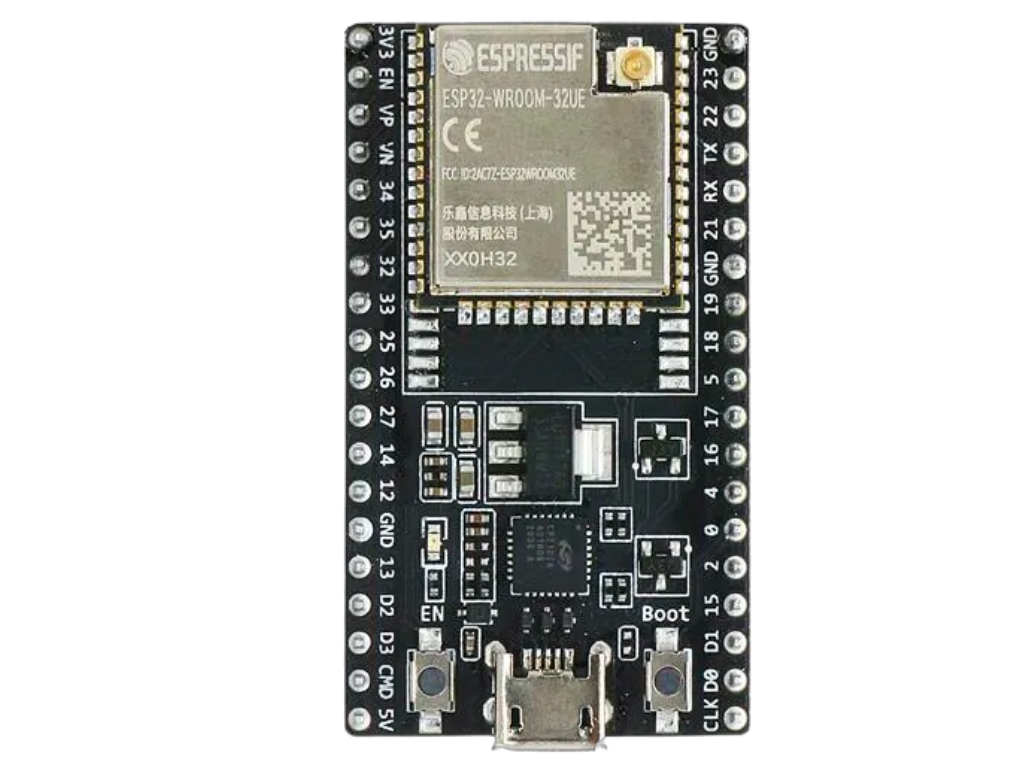
\includegraphics[width=0.4\linewidth]{assets/ch2/esp32}
	\caption{ESP32-WROOM Development board}
	\label{fig:esp32}
\end{figure}

\subsection{ESP Series Overview}

The ESP series includes different models tailored to specific application needs for performance, power efficiency, and connectivity. Key types include:

\begin{itemize}
	\item \textbf{ESP8266 Series:} A cost-effective option with a 32-bit LX6 single-core processor (up to 160 MHz), supporting 2.4 GHz Wi-Fi and peripheral interfaces like UART, I2C, and PWM. Its low power consumption suits battery-powered applications.
	
	\item \textbf{ESP32 Series:} Offers more power and connectivity. The ESP32-S2 has a single-core LX7 processor, while the ESP32-S3 features a dual-core LX7 processor (up to 240 MHz), with 2.4 GHz Wi-Fi and Bluetooth 5.0. It includes security features like secure boot and flash encryption.
	
	\item \textbf{ESP32-S2 Series:} A low-power option with a single-core LX7 processor (up to 240 MHz) and Wi-Fi support. It includes USB OTG and advanced security features, making it suitable for secure IoT applications.
	
	\item \textbf{ESP32-S3 Series:} Designed for AI and neural network applications, it features a dual-core LX7 processor (up to 240 MHz), with Wi-Fi and Bluetooth 5 (LE). It has added vector instructions for AI tasks and comprehensive security options.
\end{itemize}

\subsection{Key Features of ESP Modules}

ESP modules provide a range of features for various applications:

\begin{itemize}
	\item \textbf{Wireless Connectivity:} All modules support 2.4 GHz Wi-Fi; some also include Bluetooth 5.0 (LE).
	
	\item \textbf{Peripherals and Interfaces:} Offers GPIO, SPI, I2C, I2S, UART, PWM, ADC, DAC, and USB OTG (on select models), supporting a wide variety of sensors and devices.
	
	\item \textbf{Power Efficiency:} Low-power modes and fine-grained control make ESP modules suitable for battery-powered devices, with the ESP32-S2 optimized for ultra-low-power applications.
\end{itemize}

With their range of types, processors, and features, ESP modules offer a flexible solution for IoT and embedded systems, meeting the needs of modern, connected applications.

\section{Ultrasonic Ranging Module}



The HC-SR04 ultrasonic ranging module is a widely utilized sensor for non-contact distance measurement. Its capability to measure distances ranging from 2 cm to 400 cm, with an accuracy of up to 3 mm, makes it a versatile tool for various applications in robotics, automation, and IoT systems. This module integrates ultrasonic transmitters, a receiver, and control circuitry within a compact form factor  \cite{HCSR04Datasheet}.

\begin{figure}
	\centering
	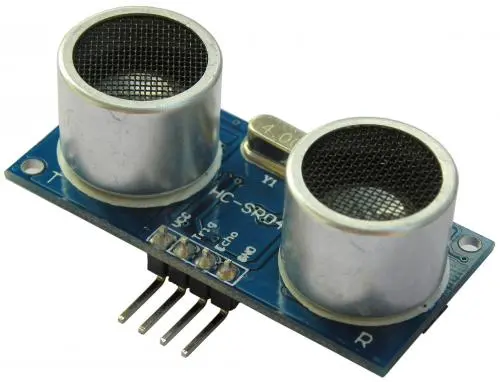
\includegraphics[width=0.4\linewidth]{assets/ch2/ultrasonic}
	\caption{HC-SR04 Module}
	\label{fig:ultrasonic}
\end{figure}


\paragraph{Working Principle}

The HC-SR04 operates by emitting an ultrasonic pulse at 40 kHz through its transmitter. This pulse propagates through the air and, upon encountering an obstacle, reflects back toward the sensor. The module measures the time taken for the echo to return to the receiver. The distance to the object can be calculated using the formula:

\[
\text{Distance} = \frac{\text{High-level time} \times \text{Speed of sound (340 m/s)}}{2}
\]

To ensure accurate results, a measurement cycle of over 60 ms is recommended to avoid interference between consecutive signals.



The HC-SR04 provides an effective and economical solution for non-contact distance measurement, with applications in diverse systems requiring proximity sensing \cite{HCSR04Datasheet}. 


\section{Coin Vibration Motor}

The C1026B Series coin vibration motor is a compact, permanent-magnetic DC motor designed for generating tactile feedback through vibrations. Its small size and high efficiency make it ideal for applications in wearable devices, handheld electronics, and consumer gadgets.

\begin{figure}[h]
	\centering
	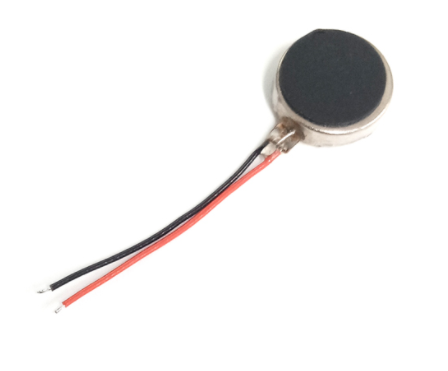
\includegraphics[width=0.4\linewidth]{assets/ch2/vibration_motor}
	\caption{C1026B Series Coin Vibration Motor}
	\label{fig:coin_motor}
\end{figure}

\paragraph{Operating Conditions}
The motor operates effectively within a voltage range of 2.7 V to 3.3 V DC, with a rated voltage of 3.0 V DC. It can function in environmental conditions ranging from -20°C to 60°C with ordinary humidity, making it robust for various settings. 

\paragraph{Working Principle}
The vibration is generated by the rapid rotation of an eccentric mass attached to the motor shaft. When powered, the imbalance caused by this mass induces vibrations, which are transmitted to the device housing the motor. This principle is commonly used in applications requiring tactile feedback or silent alerts.

\paragraph{Performance Characteristics}
The motor achieves a rated speed of 9,000 RPM at its rated voltage while consuming a maximum current of 90 mA. It is designed to start at a voltage as low as 2.3 V DC. With a mechanical noise limit of 50 dB(A), it ensures quiet operation.



The C1026B Series motor provides a reliable and efficient solution for haptic feedback and vibration alert mechanisms in compact electronic devices \cite{VybronicsVC0820B006F}.
